\section{Komponentendiagramm}

Für eine klare funktionale Übersicht auf unserer Diplomarbeit
wurde ein sogenanntes Komponentendiagramm für das technische System von Relaxoon erstellt.
Da Relaxoon eine Applikation ist, die auf Handys laufen soll,
wurde für die Entwicklung die cross plattformige \textbf{J}ava\textbf{S}cript  (js)
Framework "React Native" verwendet. Damit der Kunde Inhalte in die App hinzufügen kann,
wurde ein "Node js" basiertes Headless \textbf{C}ontent \textbf{M}anagement \textbf{S}ystem (CMS)
namens “Strapi” verwendet.
Dieses bietet eine vorgefertigte Benutzeroberfläche für die Content Creators
und auch für die Entwickler, sodass man Inhalte und dazu gebrauchte technische Funktionalitäten, wie zum Beispiel
\textbf{RE}presentational \textbf{S}tate \textbf{T}ransfer (REST)- bzw. \textbf{G}raph \textbf{Q}uery \textbf{L}anguage (Graphql)-Schnittstellen
für die Authentifizierung und \textbf{C}reate, \textbf{R}ead, \textbf{U}pdate und \textbf{D}elete (CRUD)
Funktionalitäten jeder Business Entität, sehr einfach erstellen kann.
Für die Kommunikation zwischen Frontend und Backend wird REST verwendet. Das Backend holt sich die Daten mit Hilfe eines postgresql Treibers aus der Datenbank.


\begin{figure}[H]
    \centering
    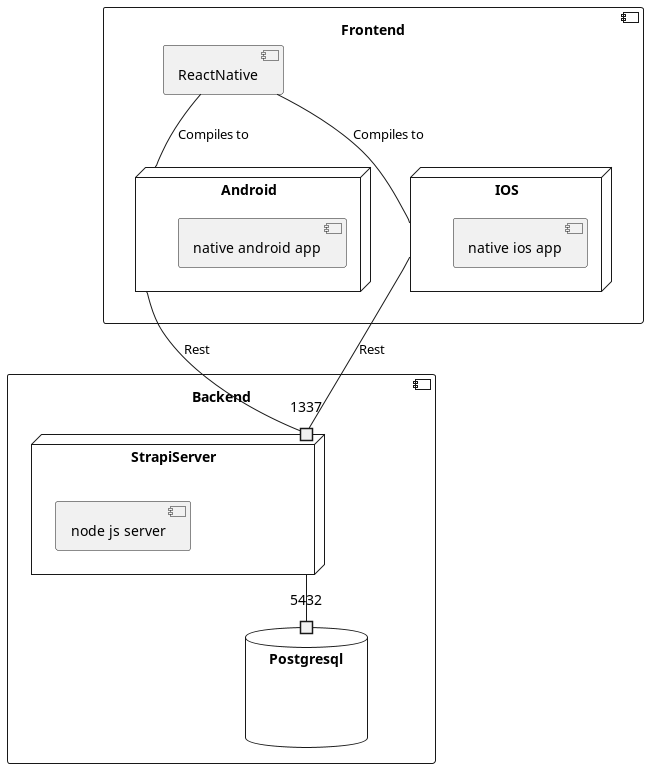
\includegraphics{./pics/system-architektur.png}
    \caption{Systemarchitektur}
    \label{fig:Systemarchitektur}
\end{figure}